\chapter{Fast Integer Matrix Multiplication}
\label{chapter:fastMM}

In this chapter, we describe and implement an algorithm for fast multiplication of matrices with 
integer entries of arbitrary length. Assume that we are able to multiply matrices with machine level 
integer entries efficiently. Then the idea is to find a multiplication preserving mapping that 
enables us to uniquely represent matrices with big entries by matrices with machine level entries. 
This mapping and its inverse should be efficiently computable. To this end, we present the modular 
representation technique for matrices. This is not a new idea, e.g. see \cite{Knuth1988} for the 
modular representation technique for arithmetic on large integers. We first describe the method, and 
then propose some practical improvements to it. In the last section, we describe two computational 
problems: modular composition, and power projection. We show how the new implementations of the 
solutions to these problems, based on the fast matrix multiplication, lead to major speed-ups.









\section{Modular representation}
\label{section:mrep}

Let $R$ be a commutative ring with 1 and let $I_1, I_2, \dots, I_k$ be ideals of $R$. Then there is 
a natural homomorphism
$$
\setlength\arraycolsep{2pt}
\renewcommand{\arraystretch}{1.25}
\begin{array}{llll}
\varphi : & R & \longrightarrow & \bigoplus_{m = 1}^k {R/I_m} \\
& a & \longmapsto & (a + I_1, a + I_2, \cdots, a + I_k)
\end{array}
$$
If the ideals $I_m$ are pairwise coprime i.e. $I_i + I_j = R$ whenever $i \ne j$ then $\varphi$ is 
surjective with kernel $\prod_{m = 1}^k {I_m}$ so that 
$$
\psi : R/\prod_{m = 1}^k {I_m} \longrightarrow \bigoplus_{m = 1}^k {R/I_m}
$$
is an isomorphism \cite{Atiyah1969}. Therefore, every element $a$ in the left side ring can be 
uniquely represented as a $k$-tuple $(a_1, a_2, \cdots, a_k)$ in the right side ring. The $k$-tuple 
$(a_1, a_2, \cdots, a_k)$ is called the modular representation of $a$. Computing $\psi$ is not 
usually computationally hard. One can compute $\psi^{-1}$ as follows. Let $M_i = \prod_{j \ne i} 
{I_j}$. Then $I_i$ and $M_i$ are coprime. So, there are $x_i \in I_i, y_i \in M_i$ such that $x_i + 
y_i = 1$. Then $1 - y_i \in I_i$ and $y_i \in M_i \subseteq I_j$ for all $j \ne i$. Now let $a = 
\sum_{m = 1}^k {a_my_m}$. It can be easily seen that $\varphi(a) = (a_1, a_2, \cdots, a_k)$. 
Therefore, multiplication in $R/\prod_{m = 1}^k {I_m}$ can be carried out by multiplication in 
$\bigoplus_{m = 1}^k {R/I_m}$ via the mapping $\psi$. This is done by 
\refalgorithm{algorithm:labsMul}.

\begin{algorithm}
[Multiplication in $R/\prod_{m = 1}^k {I_m}$]
\label{algorithm:labsMul}
\begin{algorithmic}[1]
\REQUIRE $a, b \in R/\prod_{m = 1}^k {I_m}$
\ENSURE  the product $ab$
\STATE $(a_1, \cdots, a_k) \leftarrow \psi(a)$
\STATE $(b_1, \cdots, b_k) \leftarrow \psi(b)$
\STATE compute $(a_1b_1, \cdots, a_kb_k)$
\RETURN $\psi^{-1}(a_1b_1, \cdots, a_kb_k)$
\end{algorithmic}
\end{algorithm}

Let $M_n(R)$ be the ring of $n \times n$ square matrices over $R$. The mapping $\psi$ induces the 
isomorphism
$$
\setlength\arraycolsep{2pt}
\begin{array}{llll}
\Psi : & M_n(R/\prod_{m = 1}^k {I_m}) & \longrightarrow & \bigoplus_{m = 1}^k M_n(R/I_m)\\
& (a_{ij}) & \longmapsto & (([a + I_1]_{ij}), ([a + I_2]_{ij}), \cdots, ([a + I_k]_{ij}))
\end{array}
$$
where $([a + I_r]_{ij})$ is the matrix $(a_{ij})$ with entries reduced modulo $I_r$. This means we 
can have a multiplication algorithm similar to \refalgorithm{algorithm:labsMul} in $M_n(R/\prod_{m = 
1}^k {I_m})$.

\begin{algorithm}
[Multiplication in $M_n(R/\prod_{m = 1}^k {I_m})$]
\label{algorithm:labsMMul}
\begin{algorithmic}[1]
\REQUIRE $A, B \in M_n(R/\prod_{m = 1}^k {I_m})$
\ENSURE  the product $AB$
\STATE $(A_1, \cdots, A_k) \leftarrow \Psi(A)$
\label{step:Mn-reduction1}
\STATE $(B_1, \cdots, B_k) \leftarrow \Psi(B)$
\label{step:Mn-reduction2}
\STATE compute $(A_1B_1, \cdots, A_kB_k)$
\label{step:Mn-resmul}
\RETURN $\Psi^{-1}(A_1B_1, \cdots, A_kB_k)$
\label{step:Mn-inverse}
\end{algorithmic}
\end{algorithm}

Now, consider the special case $R = \vmathbb{Z}$. In this case, the ideals are principal and 
computing $\psi$, and $\psi^{-1}$ reduces to the usual modular integer operations. Let $I_i = (p_i), 
\: i = 1, \dots, k$ with $p_i$ prime; Then computing $\psi^{-1}$ is equivalent to solving the system 
of congruences $x \equiv a_ib_i \pmod {p_i}, \: i = 1, \dots, k$ which can be done as follows. Let 
$M = \prod_{i = 1}^k p_i$, and $M_i = M / p_i$. Compute $t_i = M_i^{-1} \pmod {p_i}$. Then $x  = 
\sum_{i = 1}^k a_it_iM_i \pmod M$ (see \refalgorithm{algorithm:lZMul}). Since $\vmathbb{Z}$ is a 
normed ring, we can talk about the sizes of the elements so that  \refalgorithm{algorithm:labsMul} 
can be used in the following way. Let $a, b \in \vmathbb{Z}$ be of arbitrary length. Chose $p_i$ such 
that $a_i$ and $b_i$ fit into machine words. Compute machine level products $(a_1b_1, \cdots, 
a_kb_k)$, and finally compute $\psi^{-1}(a_1b_1, \cdots, a_kb_k)$ by \refalgorithm{algorithm:lZMul}.

Accordingly, \refalgorithm{algorithm:labsMMul} can be used in a similar way to multiply integer 
matrices. It first reduces matrices $A, B$ to tuples $(A_1, \cdots, A_k), (B_1, \cdots, B_k)$ of 
matrices with entries that can fit into machine words. It then computes the matrix products 
$(A_1B_1, \cdots, A_kB_k)$ and at last $\Psi^{-1}(A_1B_1, \cdots, A_kB_k)$ by applying 
\refalgorithm{algorithm:lZMul}
to corresponding entries of the matrices $A_iB_i$. In the case of matrices, the values $M$ and $M_i$ 
can be precomputed for the entire process. We shall discuss  some optimization techniques in 
\refsection{section:impl}.

\begin{algorithm}
[Computing $\psi^{-1}$ in $\vmathbb{Z}$]
\label{algorithm:lZMul}
\begin{algorithmic}[1]
\REQUIRE $(a_1, \cdots, a_k) \in \bigoplus_{i = 1}^k \vmathbb{Z}_{p_i}$
\ENSURE  $a \in \vmathbb{Z}$
\STATE $M \leftarrow \prod_{i = 1}^k p_i$
\FOR{$i$ from $1$ to $k$}
	\STATE $M_i \leftarrow \prod_{j \ne i} p_i$
\ENDFOR
\FOR{$i$ from $1$ to $k$}
\label{step:gauss-minv}
	\STATE $t_i \leftarrow M_i^{-1} \mod {p_i}$
	\STATE $x \leftarrow x + a_it_iM_i$
\ENDFOR
\RETURN $x \mod M$
\end{algorithmic}
\end{algorithm}










\section{Implementation}
\label{section:impl}

The algorithm described in \refsection{section:mrep} for multiplication of integer matrices has been 
implemented and embedded into the NTL library \cite{NTL2009}. It is a low level implementation with 
high level interfaces. For both compatibility and handling low level fast big integer arithmetic, 
the GMP library \cite{GMP2010} is used. For multiplication of matrices with machine level entries, 
ATLAS library \cite{ATLAS2010} is used. A simple parallelism scheme is used, which results in an 
essentially linear speed up. The number of processors the algorithm is allowed to use can be set for 
each call; otherwise, it uses all processors of the system. Various techniques, with different 
performances depending on the shapes of the inputs, for computing $\Psi^{-1}$ have been implemented 
so one can set the computation mode for each call. Figure \ref{figure:MMtiming} compares the running 
times of the proposed matrix multiplication, in sequential mode, and the one built in Magma 
\cite{Magma2010} on a Core 2 Quad machine. \footnote{Magma, which probably uses the same idea for 
matrix multiplication, is apparently the fastest computer algebra system in this respect.}

\begin{figure}[ht]
\setlength{\abovecaptionskip}{-0.5cm}
%\setlength{\belowcaptionskip}{0cm}
\begin{center}
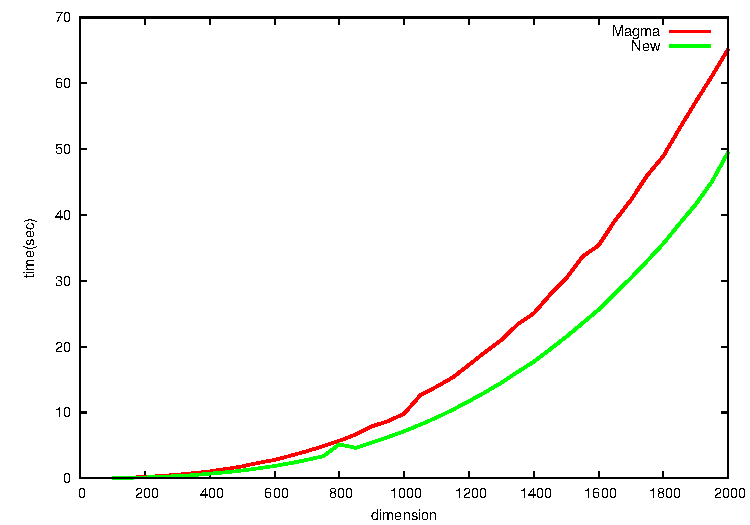
\includegraphics[width = 10cm]{figures/MMtiming.pdf}
\end{center}
\caption{\small Matrix multiplication with bitsize 200}
\label{figure:MMtiming}
\end{figure}

A natural way of computing $\Psi$ is to simply iterate over all entries of the input matrix and 
reduce each entry module each prime $p_i$ by a fast reduction function. But a more clever way is to 
do reduction by matrix multiplication as follows. Let $v = (t_1, t_2, \cdots, t_n)$ be a row of the 
matrix $A$. Write $t_i = t_{i1}t_{i2}\cdots t_{ir}$ in a basis of the form $\omega = 2^d$. Then 
compute
\[
C = 
 \begin{pmatrix}
  \omega^r \pmod {p_1} & \omega^{r - 1} \pmod {p_1} & \cdots &  1\\
  \omega^r \pmod {p_2} & \omega^{r - 1} \pmod {p_2} & \cdots &  1\\
  \vdots  & \vdots  & \ddots & \vdots  \\
  \omega^r \pmod {p_k} & \omega^{r - 1} \pmod {p_k} & \cdots &  1\\
 \end{pmatrix}
 \begin{pmatrix}
  t_{11} & t_{21} & \cdots & t_{n1} \\
  t_{12} & t_{22} & \cdots & t_{n2} \\
  \vdots  & \vdots  & \ddots & \vdots  \\
  t_{1r} & t_{2r} & \cdots & t_{nr} \\
 \end{pmatrix}
\]
The $i$th, $1 \le i \le k$, row of the matrix $C$ is the row $v$ reduced mod $p_i$. The same thing 
can be done for all rows of $A$ to compute the tuple $(A_1, \dots, A_k)$. The Vandermonde like 
matrix of $\omega^i$ is precomputed.

If the entries of the input matrices are very large then the value $x = \sum_{i = 1}^k a_it_iM_i$ in 
\refstep{step:gauss-minv} of  \refalgorithm{algorithm:lZMul} can be computed by a divide and conquer 
algorithm \cite{VonzurGathen1999}: Let $\alpha = p_{k / 2 + 1}p_{k / 2 + 2}\cdots p_k$ and $\beta = 
p_1p_2\cdots p_{k / 2}$ then
\begin{eqnarray*}
x & = & \alpha(a_1t_1M_1/\alpha + \cdots + a_{k / 2}t_{k / 2}M_{k / 2}/\alpha) \\
& & + \beta(a_{k / 2 + 1}t_{k / 2 + 1}M_{k / 2 + 1}/\beta + \cdots + a_kt_kM_k/\beta)
\end{eqnarray*}
All the values $\alpha$ and $\beta$ are precomputed. Another way of computing $x = \sum_{i = 1}^k 
a_it_iM_i$ is using a similar matrix multiplication technique as above with $t_i$ replaced by $M_i$. 
Figure \ref{figure:MMtimingDetail} shows a timing for different phases of 
\refalgorithm{algorithm:labsMMul} where \verb|reduction|, \verb|residue mul|, and \verb|inverse| are 
steps \{\ref{step:Mn-reduction1}, \ref{step:Mn-reduction2}\}, \ref{step:Mn-resmul}, and 
\ref{step:Mn-inverse} of the algorithm respectively.

\begin{figure}[ht]
\setlength{\abovecaptionskip}{-0.5cm}
%\setlength{\belowcaptionskip}{0cm}
\begin{center}
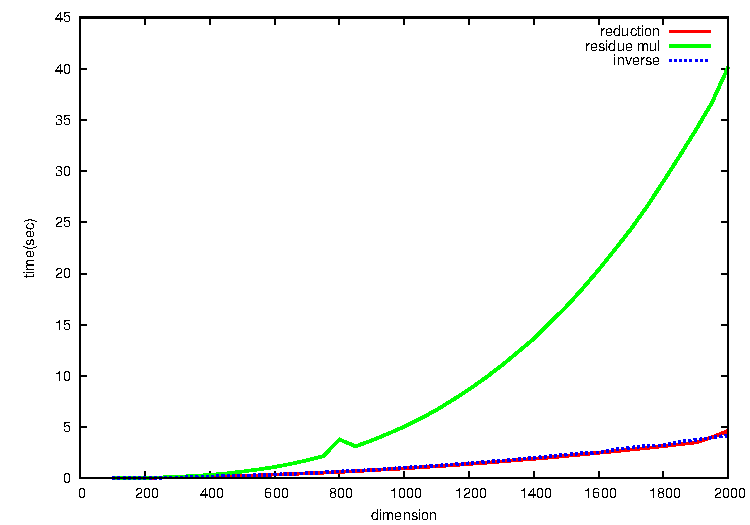
\includegraphics[width = 10cm]{figures/MMtimingDetail.pdf}
\end{center}
\caption{\small Multiplication phases with bitsize 200}
\label{figure:MMtimingDetail}
\end{figure}










\section{Some computational speed-ups}
\label{section:MMapll}

Matrix multiplication is the building block of many computational algorithms. Therefore, having a 
fast matrix multiplication library results in a speed-up in many computational areas. In this 
section, we present some specific problems, required in subsequent chapters, and show how to have 
major speed-ups by giving new implementations of the solutions based on matrix multiplication.

\paragraph{Modular Polynomial Composition.}
Let $F$ be a field and let $p(x) = p_0 + p_1x + \cdots + p_nx^n$, $q(x) = q_0 + q_1x + \cdots + 
q_nx^n$, and $f(x)$ be polynomials in $F[x]$. Then the problem is to compute $p(q) \text{ mod } f$. 
Here, we implement an algorithm by Brent and Kung \cite{BreKun1978} which was proposed for 
computation of the first $n \in \vmathbb{N}_{\ge 1}$ coefficients of the composition of two formal 
power series. But it also works for polynomial composition modulo an arbitrary polynomial $f(x)$.
\begin{algorithm}
[Modular Polynomial Composition]
\label{algorithm:polyComp}
\begin{algorithmic}[1]
\REQUIRE  polynomials $p, q, f \in F[x]$
\ENSURE  $q(p) \text{ mod } f$
\STATE $k \leftarrow \lceil \sqrt{n + 1} \rceil$
\STATE write $q(x) = Q_0(x) + Q_1(x)x^k + \cdots + Q_{k - 1}(x)(x^k)^{k - 1}$
\STATE compute $p^i(x), \: i = 2, \dots, k$
\label{step:BK-pi}
\STATE let $T(s) = p^k(x)$ and compute $T^i(x), \: i = 2, \dots, k - 1$
\label{step:BK-Ti}
\STATE compute $Q_i(p(x)), \: i = 0, \dots, k - 1$ from the \refstep{step:BK-pi}.
\label{step:BK-Qi}
\STATE compute $Q_i(p(x))T^i(x), \: i = 1, \dots, k - 1$ from the steps \ref{step:BK-Ti} and 
\ref{step:BK-Qi}.
\label{step:BK-QiTi}
\STATE compute $h(x) = \sum_{i = 0}^{k - 1} Q_i(p(x))T^i(x)$ from \refstep{step:BK-QiTi}.
\RETURN $h(x)$
\end{algorithmic}
\end{algorithm}
Note that all computations of \refalgorithm{algorithm:polyComp} are done modulo $f(x)$. Let $p^j(x) 
= \sum_{l = 0}^n p_l^{(j)}x^l$, $j = 0, \dots, k$. Then 
$$
Q_i(p(x)) = \sum_{j = 0}^{k - 1} q_{ik + j} \sum_{l = 0}^n p_l^{(j)}x^l = \sum_{l = 0}^n \left(  
\sum_{j = 0}^{k - 1} q_{ik + j}p_l^j\right)x^l
$$
which is essentially the following matrix multiplication.
\[
 \begin{pmatrix}
  p_0^{(0)} & p_0^{(1)} & \cdots & p_0^{(k - 1)} \\
  p_1^{(0)} & p_1^{(1)} & \cdots & p_1^{(k - 1)} \\
  \vdots  & \vdots  & \ddots & \vdots  \\
  p_n^{(0)} & p_n^{(1)} & \cdots & p_n^{(k - 1)}
 \end{pmatrix}
 \begin{pmatrix}
  q_0 & q_k & \cdots & q_{(k - 1)k} \\
  q_1 & q_{k + 1} & \cdots & q_{(k - 1)k + 1} \\
  \vdots  & \vdots  & \ddots & \vdots  \\
  q_{k - 1} & q_{2k - 1} & \cdots & q_{k^2 - 1}
 \end{pmatrix}
\]

\begin{figure}[ht]
\setlength{\abovecaptionskip}{-0.5cm}
%\setlength{\belowcaptionskip}{0cm}
\begin{center}
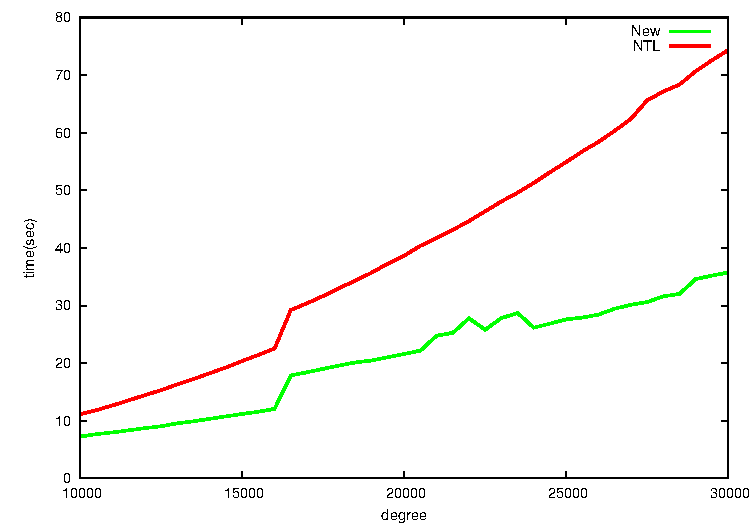
\includegraphics[width = 10cm]{figures/polyCompTiming.pdf}
\end{center}
\caption{\small Modular Polynomial Composition}
\label{figure:polyCompTiming}
\end{figure}

Therefore, \refstep{step:BK-Qi} of \refalgorithm{algorithm:polyComp} can be done using matrix 
multiplication. Let assume that $O(n^\omega)$ is the achievable bound for multiplication of two $n 
\times n$ matrices. For the classical matrix multiplication $\omega = 3$, and for the best known 
algorithm $\omega = 2.37$ \cite{Coppersmith1990}. Except \refstep{step:BK-Qi}, all steps of the 
algorithm can be done in $O(kM(n)) = O(\sqrt{n}M(n))$ multiplications in $F$. Multiplication of the 
matrices of size $n \times \sqrt{n}$ and $\sqrt{n} \times \sqrt{n}$ in \refstep{step:BK-Qi} is 
indeed equivalent to $\sqrt{n}$ multiplications of square matrices of dimension $\sqrt{n} \times 
\sqrt{n}$, which can be done in $O(\sqrt{n}n^{\omega / 2}) = O(n^{(\omega + 1) / 2})$ operations in 
$F$. Therefore, the running time of \refalgorithm{algorithm:polyComp} is $O(\sqrt{n}M(n) + 
n^{(\omega + 1) / 2})$ operations in $F$. So, assuming $M(n) = O(n\log n \log\log n)$, and $\omega = 
2.37$, the best running time for modular composition is $O(n^{1.69})$.\footnote{Huang and Pan 
\cite{Huang1997} showed that for the special dimensions $\sqrt{n} \times \sqrt{n}$ times $\sqrt{n} 
\times n$, $\omega \le 1.67$. So for their algorithm $C(n) = O(n^{1.67})$.} A new implementation of 
the polynomial composition using our matrix multiplication algorithm has been embedded into NTL. 
Figure \ref{figure:polyCompTiming} compares the new and the old algorithm for modular polynomial 
composition in NTL. 

Now that we have a fast modular polynomial composition we briefly show how to use it in polynomial 
factorization over finite fields. Let us first briefly review a factorization method. Let $f(x) \in 
\vmathbb{F}_q[x]$ be of degree $n$, where $q = p^m$ and $\vmathbb{F}_q$ is represented as the quotient 
$\vmathbb{F}_p[y]/g(y)$ with $g(y) \in \vmathbb{F}_p[y]$ monic irreducible of degree $m$. An efficient 
way of factoring $f$ over $\vmathbb{F}_q$ is breaking the factoring into three steps:
\begin{enumerate}
\item \emph{squarefree factorization}: taking the square-free part of $f$;
\label{item:sqf-factor}
\item \emph{distinct-degree factorization}: splitting the square-free polynomial into polynomials 
whose irreducible factors have the same degree;
\item \emph{equal-degree factorization}: completely factoring the square-free polynomial whose 
irreducible factors have the same degree.
\end{enumerate}
The cost of \refstep{item:sqf-factor}, which is done by Yun's algorithm \cite{Yun1976}, is 
$O(M(n)\log n + n\log (q / p))$ operations in $\vmathbb{F}_q$ which is dominated by the cost of other 
steps. So, let assume $f$ is squarefree. The distinct-degree factorization is based on the fact that 
$x^{q^d} - x$ is the product of all monic irreducible polynomials of degree dividing $d$. So, taking 
$\gcd(x^{q^d} - x, f)$ isolates all factors of degree $d$ of $f$. This idea is attributed to Arwin 
\cite{Arwin1918}.

\begin{algorithm}
[Distinct-degree factorization]
\label{algorithm:DDF}
\begin{algorithmic}[1]
\REQUIRE A squarefree monic polynomial $f \in \vmathbb{F}_q[x]$ of degree $n$
\ENSURE The distinct-degree decomposition of $f$
\STATE $f_0 \leftarrow f$, $s \leftarrow \lceil \frac{n}{2} \rceil$
\FOR{$i$ from $1$ to $s$}
	\STATE $h \leftarrow x^{q^i} \text{ mod } f$
	\STATE $g_i \leftarrow \gcd(h - x, f_i)$
	\STATE $f_i \leftarrow \frac{f_{i - 1}}{g_i}$
\ENDFOR
\RETURN $(g_1, \cdots, g_s)$
\end{algorithmic}
\end{algorithm}

Each $g_i$ produced by \refalgorithm{algorithm:DDF} is a squarefree product of monic irreducible 
factors of degree $i$ of $f$. The equal-degree factorization takes $g_i$ and splits it into its 
irreducible factors. This is usually done recursively, i.e. the polynomial is split into two parts 
then the same is done for each of the two parts and so on. The idea, which is due to 
\cite{CantorandZassenhaus1981}, is as follows. Let $f \in \vmathbb{F}_q[x]$ be a squarefree monic 
polynomial of degree $n$ with $\ell = n / d$ irreducible factors $f_i, \: i = 1, \dots, \ell$ of 
degree $d$. Then
$$
\vmathbb{F}_q[x] / \langle f \rangle \cong \prod_{i = 1}^{\ell} \vmathbb{F}_q[x] / \langle f_i \rangle 
\cong \vmathbb{F}_{q^d}^\ell
$$
which induces the mapping 
$$
\setlength\arraycolsep{2pt}
\begin{array}{llll}
\sigma: & \vmathbb{F}_q[x] / \langle f \rangle & \longrightarrow & \{-2, 0\}^{\ell}\\
& a & \longmapsto & (a_1, \dots, a_{\ell})
\end{array}
$$
where $a_i = a^{(q^d - 1) / 2} - 1 \text{ mod } f_i$. Assume $\beta \in \vmathbb{F}_q[x] / \langle f 
\rangle$ is selected at random, and $\sigma(\beta) = (\beta_1, \dots, \beta_\ell)$. If $g = 
\gcd(\beta, f) \ne 1$ then $g$ is a nontrivial factor of $f$; otherwise $\gcd(\beta, f) = 1$, and 
$\gcd(\beta^{(q^d - 1) / 2} - 1, f)$ is a nontrivial factor of $f$ unless $\beta_1 = \beta_2 = 
\dots, = \beta_\ell$ \footnote{If $\beta$ is selected uniformly at random then $\beta_i = -1$ or $1$ 
with probability $1/2$. So, $\beta_1 = \beta_2 = \dots, = \beta_\ell$ occurs with probability 
$2^{-\ell + 1}$.}. 

\begin{algorithm}
[Equal-degree splitting]
\label{algorithm:EDS}
\begin{algorithmic}[1]
\REQUIRE A squarefree monic polynomial $f \in \vmathbb{F}_q[x]$ of degree $n$ and a divisor $d$ of 
$n$ such that all irreducible factors of $f$ have degree $d$.
\ENSURE a proper monic factor of $f$ or "failure"
\STATE $\beta \leftarrow$ a nonconstant random element of $\vmathbb{F}_q[x]$ of degree less than $n$
\STATE $g \leftarrow \gcd(\beta, f)$
\IF {$g \ne 1$} 
	\RETURN $g$ 
\ENDIF
\STATE $g \leftarrow \gcd(\beta^{(q^d - 1) / 2} - 1 \text{ mod } f, f)$
\label{step:EDS-main}
\IF {$g \ne 1, f$} 
	\RETURN $g$ 
\ELSE
	\RETURN "failure"
\ENDIF
\end{algorithmic}
\end{algorithm}
 
The costliest part of \refalgorithm{algorithm:EDS} is \refstep{step:EDS-main}. We show how to 
compute $\beta^{(q^d - 1) / 2} - 1 \text{ mod } f$ efficiently. Let $\lambda \in \vmathbb{F}_q[x]$, 
and assume we are asked to compute $\alpha_k = \lambda^{1 + p + p^2 + \cdots + p^k} \text{ mod } f$ 
for a given integer $k > 0$. Let $\delta_i = \lambda^{p + p^2 + \cdots + p^i} \text{ mod } f$, 
$\zeta_i = x^{p^i} \text{ mod } f$, and $\xi_i = y^{p^i}  \text{ mod } g(y)$. Then we have the 
following recurrence relations
$$
\delta_i = 
\begin{cases}
\delta_{i / 2}\delta_{i / 2}^{p^{i / 2}} & \text{if } i \overset{2}{\equiv} 0 \\
\delta_1\delta_{i - 1}^p & \text{if } i \overset{2}{\equiv} 1 \\
\delta_1 = \lambda^p
\end{cases}
\qquad
\zeta_i = 
\begin{cases}
\zeta_{i / 2}^{p^{i / 2}} & \text{if } i \overset{2}{\equiv} 0 \\
\zeta_{i - 1}^p & \text{if } i \overset{2}{\equiv} 1 \\
\zeta_1 = x^p
\end{cases}
\qquad
\xi_i =
\begin{cases}
\xi_{i / 2}^{p^{i / 2}} & \text{if } i \overset{2}{\equiv} 0 \\
\xi_{i - 1}^p & \text{if } i \overset{2}{\equiv} 1 \\
\xi_1 = y^p
\end{cases}
$$
The initial values $\delta_1$, $\zeta_1$, and $\xi_1$ are computed using the usual exponentiation 
algorithm at a total cost of $O(M(n)M(m)\log p)$ operations in $\vmathbb{F}_p$. Assume, inductively, 
that we have computed $\delta_r$, $\zeta_r$, and $\xi_r$. Then 
\begin{align*}
\delta_r^{p^r} = \left( \sum_{j = 0}^{n - 1} a_j(y)x^j \right)^{p^r} 
& = \sum_{j = 0}^{n - 1} a_j(y)^{p^r}(x^j)^{p^r} = \sum_{j = 0}^{n - 1} a_j(y^{p^r})(x^{p^r})^j\\
& = \sum_{j = 0}^{n - 1} a_j(\xi_r)\zeta_r^j \text{ mod } \langle f(x), g(y) \rangle
\end{align*}
This means that $\delta_{2r}$ and $\delta_{2r + 1}$ can be computed using $O(n)$ modular 
compositions over $\vmathbb{F}_p$, which totally costs $O(nC(m))$ operations in $\vmathbb{F}_p$, and 
$O(1)$ modular multiplications and modular compositions over $\vmathbb{F}_q$, which totally costs 
$O(C(n)M(m))$ operations in $\vmathbb{F}_p$. The values $\zeta_{2r}$ and $\zeta_{2r + 1}$ are 
computed similarly. The cost of computing $\xi_{2r}$ and $\xi_{2r + 1}$ is dominated by the above. 
Therefore, $\delta_k$ and hence $\alpha_k = \lambda\delta_k$ can be computed using $O(\log 
k(M(n)M(m)\log p + nC(m) + C(n)M(m)))$ operations in $\vmathbb{F}_p$. Now, let $\lambda = \beta^{(p - 
1) / 2}$ then
$$
\beta^{(q^d - 1) / 2} = \beta^{(p^{md} - 1) / 2} = \left( \beta^{(p - 1) / 2} \right)^{1 + p + p^2 + 
\cdots + p^{md - 1}} = \lambda^{1 + p + p^2 + \cdots + p^{md - 1}} \text{ mod } \langle f(x), g(y) 
\rangle
$$
which can be computed at a cost of $O(\log(md)(M(n)M(m)\log p + nC(m) + C(n)M(m)))$ operations in 
$\vmathbb{F}_p$. The above idea of using modular composition for raising to the powers of the 
characteristic is essentially due to Kaltofen and Shoup \cite{KaltofenShoup1997}.

To speed the distinct-degree factorization up, \refalgorithm{algorithm:DDF}, the values $x^q, 
x^{q^2}, \dots, x^{q^s}$ can be computed at once. For this, we first compute $x^q = x^{p^m}$ using 
the above algorithm and then compute $x^{q^2}, \dots, x^{q^s}$ using the algorithm introduced in 
\cite{zurShoup1992}. 

\paragraph{Power Projection.}
Let $f \in \vmathbb{F}_p[x]$ with $\deg f = n$. Given $g \in \vmathbb{F}_p[x]/(f)$, and the vector $v 
\in \vmathbb{F}_p^n$, the problem is to compute the sequence
\begin{equation}
\label{equation:powp}
\langle v, 1\rangle, \langle v, g\rangle , \dots, \langle v, g^{m - 1} \rangle
\end{equation}
for a positive integer $m$; Here, $\langle ., .\rangle$ is the inner product operator. Let $h\circ v 
\in \vmathbb{F}_p^n$ be the unique vector such that $\langle h\circ v, \alpha \rangle = \langle v, 
h\alpha \rangle$ for all $\alpha \in \vmathbb{F}_p[x]/(f)$. Sequence (\ref{equation:powp}) can be 
computed by \refalgorithm{algorithm:powerp} due to Shoup \cite{Shoup1999}. \refstep{step:powerp-for} 
of the algorithm can be replaced by a matrix multiplication. As in the case of polynomial 
composition, this new power projection algorithm has been embedded into NTL. Figure 
\ref{figure:powerp} compares the performance of the old and the new algorithm.

\begin{algorithm}
[Power Projection]
\label{algorithm:powerp}
\begin{algorithmic}[1]
\REQUIRE  $v \in \vmathbb{F}_p^n, f  \in \vmathbb{F}_p[x], g \in \vmathbb{F}_p[x]/(f)$
\ENSURE   The sequence $\langle v, 1\rangle, \langle v, g\rangle , \dots, \langle v, g^{m - 1} 
\rangle$
\STATE $k \leftarrow \lfloor l^{1/2} \rfloor, \: k^\prime \leftarrow \lceil l/k \rceil$
\FOR{$i$ from $0$ to $k^\prime - 1$}
\label{step:powerp-for}
	\STATE $c_{ik + j} \leftarrow \langle v, g^j\rangle \quad (0 \le j < k)$
	\STATE $v \leftarrow g^k \circ v$
\ENDFOR
\RETURN $c_0, \dots, c_{m - 1}$
\end{algorithmic}
\end{algorithm}

\begin{figure}[ht]
\setlength{\abovecaptionskip}{-0.5cm}
%\setlength{\belowcaptionskip}{0cm}
\begin{center}
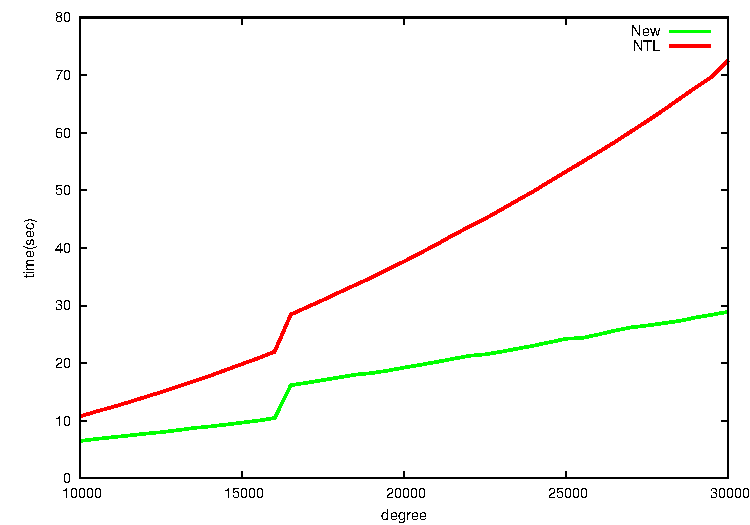
\includegraphics[width = 10cm]{figures/powerProjectTiming.pdf}
\end{center}
\caption{\small Power Projection}
\label{figure:powerp}
\end{figure}


